% Copyright (c) 2026 CorrectBrain
% SPDX-License-Identifier: MIT

\PassOptionsToPackage{dvipsnames,svgnames,x11names}{xcolor}
\documentclass[tikz,border=8pt]{standalone}
\usetikzlibrary{arrows.meta,positioning,calc,shapes,shadows,decorations.pathmorphing,shapes.geometric,backgrounds,decorations.markings,decorations.pathreplacing,decorations.text,fit,shapes.misc,shapes.arrows,matrix,bending,3d,chains,intersections,shapes.symbols,svg.path,shapes.multipart,snakes,shapes.callouts,angles,quotes,fadings,shadows.blur,patterns,patterns.meta}

\providecolor{gold}{RGB}{212,175,55}
\providecolor{silver}{RGB}{192,192,192}
\providecolor{bronze}{RGB}{205,127,50}
\providecolor{darkblue}{RGB}{0,0,139}
\providecolor{lightblue}{RGB}{173,216,230}
\providecolor{darkgreen}{RGB}{0,100,0}
\providecolor{lightgreen}{RGB}{144,238,144}
\providecolor{darkred}{RGB}{139,0,0}
\providecolor{navy}{RGB}{0,0,128}
\providecolor{skyblue}{RGB}{135,206,235}
\providecolor{beige}{RGB}{245,245,220}
\providecolor{cream}{RGB}{255,253,208}

\usepackage{amsmath}
\usepackage{amssymb}
\usepackage{fontawesome5}

% --- COLOR PALETTE DEFINITIONS ---
\definecolor{viewportdark}{HTML}{005A9C}
\definecolor{viewportlight}{HTML}{0078D7}
\definecolor{copperdark}{HTML}{B87333}
\definecolor{copperlight}{HTML}{D4AF37}
\definecolor{codebg}{HTML}{1E1E1E}
\definecolor{codeheader}{HTML}{2D2D2D}
\definecolor{syntaxblue}{HTML}{9CDCFE}
\definecolor{syntaxyellow}{HTML}{CE9178}
\definecolor{syntaxpurple}{HTML}{C586C0}
\definecolor{macred}{HTML}{FF5F56}
\definecolor{macyellow}{HTML}{FFBD2E}
\definecolor{macgreen}{HTML}{27C93F}
\definecolor{slate}{HTML}{475569}
\definecolor{slatelight}{HTML}{F8FAFC}
\definecolor{mathgreen}{RGB}{46, 125, 50}
\definecolor{targetpurple}{RGB}{123, 31, 162}
\definecolor{textdark}{RGB}{28, 28, 28}
\definecolor{hworange}{RGB}{230, 115, 0}
\definecolor{viewportblue}{RGB}{0, 120, 215}

\begin{document}
\begin{tikzpicture}[
    % --- COMPONENT STYLES ---
    bubble/.style={
        draw=black!15, fill=white, rounded corners=8pt,
        inner sep=12pt, blur shadow={shadow opacity=20, shadow yshift=-3pt, shadow xshift=0pt, shadow blur steps=10}
    },
    titlebox/.style={
        fill=white, draw=black!12, rounded corners=10pt,
        inner sep=14pt, blur shadow={shadow opacity=20, shadow yshift=-3pt, shadow xshift=0pt, shadow blur steps=10}
    },
    viewportcard/.style={
        top color=viewportdark, bottom color=viewportlight, text=white,
        draw=viewportdark!80, line width=1pt, rounded corners=8pt,
        inner sep=12pt, blur shadow={shadow opacity=25, shadow yshift=-3pt, shadow xshift=0pt, shadow blur steps=10}
    },
    hardwarecard/.style={
        top color=copperlight!30, bottom color=copperdark!20, text=textdark,
        draw=copperdark, line width=1.2pt, rounded corners=8pt,
        inner sep=12pt, blur shadow={shadow opacity=20, shadow yshift=-3pt, shadow xshift=0pt, shadow blur steps=10}
    },
    macwindow/.style={
        fill=codebg, draw=black!40, line width=0.8pt, rounded corners=7pt,
        inner sep=0pt, blur shadow={shadow opacity=25, shadow yshift=-3pt, shadow xshift=0pt, shadow blur steps=10}
    },
    enginebox/.style={
        draw=slate!40, dashed, line width=1.5pt, fill=slatelight, rounded corners=12pt
    },
    arrow/.style={
        -Stealth=3mm, line width=2pt, color=slate, rounded corners=5pt
    },
    matharrow/.style={
        -Stealth=3mm, line width=2.5pt, color=mathgreen, rounded corners=5pt
    },
    dataarrow/.style={
        -Stealth=3mm, line width=2.5pt, color=copperdark, rounded corners=5pt
    },
    circuitdot/.style={
        circle, fill=slate!80, inner sep=0pt, minimum size=5pt
    }
]

% --- 1. TITLE NODE (0, 20.5) ---
\node[titlebox, text width=16.5cm, align=center] (titlenode) at (0, 20.5) {
    {\Huge\bfseries\color{textdark} Phase 1: Spatial Target Calculation}\\[5pt]
    {\large\color{gray!90}How the rendering engine translates fluid CSS \texttt{sizes} and hardware DPR into a physical target.}
};

% --- 2. TOP INPUT LAYER (Y = 16.5) ---

% Viewport Input (-12.5, 16.5)
\node[viewportcard, text width=5.2cm, align=center] (viewport) at (-12.5, 16.5) {
    {\Large\color{white}\faDesktop}\\[5pt]
    {\large\textbf{Current Viewport (vw)}}\\[4pt]
    {\small User resized the window to:}\\[3pt]
    {\LARGE\textbf{1200px}} wide
};

% Code Editor Window Input (0, 16.5)
\node[macwindow, text width=11cm, align=center] (codebox) at (0, 16.5) {
    % Window Header Bar
    \begin{tikzpicture}[baseline=(header.south)]
        \fill[codeheader, rounded corners=7pt] (-5.5, 0) rectangle (5.5, 0.7);
        \fill[codeheader] (-5.5, 0) rectangle (5.5, 0.3); % Square off bottom edge
        \fill[macred] (-5.1, 0.35) circle (3pt);
        \fill[macyellow] (-4.8, 0.35) circle (3pt);
        \fill[macgreen] (-4.5, 0.35) circle (3pt);
        \node (header) [font=\footnotesize\bfseries\color{gray!40}, anchor=center] at (0, 0.35) {\faCode\ HTML Parser Source};
    \end{tikzpicture}\\[4pt]
    % Code Body with Syntax Highlighting
    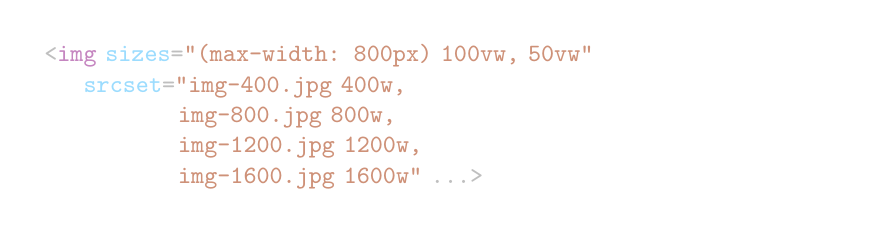
\begin{tikzpicture}
        \node[font=\ttfamily\small, text width=10.2cm, align=left, text=white, inner sep=6pt] {
            \textcolor{gray!50}{<}\textcolor{syntaxpurple}{img} \textcolor{syntaxblue}{sizes}\textcolor{gray!50}{=}\textcolor{syntaxyellow}{"(max-width: 800px) 100vw, 50vw"}\\
            \hspace*{0.5cm}\textcolor{syntaxblue}{srcset}\textcolor{gray!50}{=}\textcolor{syntaxyellow}{"img-400.jpg 400w,}\\
            \hspace*{1.7cm}\textcolor{syntaxyellow}{img-800.jpg 800w,}\\
            \hspace*{1.7cm}\textcolor{syntaxyellow}{img-1200.jpg 1200w,}\\
            \hspace*{1.7cm}\textcolor{syntaxyellow}{img-1600.jpg 1600w"} \textcolor{gray!50}{...>}
        };
    \end{tikzpicture}
    \vspace{4pt}
};

% --- 3. HARDWARE DPR INPUT LAYER (Moved to Middle-Left: -12.5, 2.5) ---
\node[hardwarecard, text width=5.2cm, align=center] (hardware) at (-12.5, 2.5) {
    {\Large\color{copperdark}\faMicrochip}\\[5pt]
    {\large\textbf{Device Pixel Ratio (DPR)}}\\[4pt]
    {\small High-density Retina Display:}\\[3pt]
    {\LARGE\textbf{2.0x}} multiplier
};

% --- 4. BROWSER RENDERING ENGINE PIPELINE NODES (Centered at X = 0) ---

% Engine Step 1: Media Query Evaluation (0, 10.5)
\node[bubble, text width=13cm, fill=white, draw=viewportdark!40, line width=1.1pt, scale=0.8] (sizesengine) at (0, 10.5) {
    {\large\textbf{\textcolor{viewportdark}{\faCog\ Engine Step 1: Media Query Evaluation}}}\\[7pt]
    The browser evaluates the \texttt{sizes} list strictly from left to right against the Viewport (1200px).\\[6pt]
    \begin{tabular}{p{5.5cm} p{1cm} p{4.5cm}}
        \textbf{Condition 1:} \texttt{(max-width: 800px)} & $\rightarrow$ & \textcolor{red}{\textbf{FALSE}} (1200 $\not\le$ 800) \\
        \textbf{Condition 2 (Default):} \texttt{50vw} & $\rightarrow$ & \textcolor{mathgreen}{\textbf{TRUE}} (Fallback match) \\
    \end{tabular}\\[7pt]
    \textit{Conclusion: The image will occupy \textbf{50\% of the viewport width} in CSS layout space.}
};

% CSS Pixel Translation (0, 6.5)
\node[bubble, text width=10.5cm, align=center, draw=mathgreen, line width=1.2pt, scale=0.8] (cssmath) at (0, 6.5) {
    {\large\textbf{\textcolor{mathgreen}{\faCalculator\ CSS Pixel Translation}}}\\[5pt]
    50vw mathematically translates to:\\[2pt]
    $0.5 \times 1200\text{px (Viewport)}$ = \textbf{\LARGE 600px}\\[4pt]
    \small\textit{(This is the predicted spatial layout size)}
};

% Engine Step 2: Hardware Augmentation (0, 2.5)
\node[bubble, text width=12cm, align=center, fill=copperlight!10, draw=copperdark, line width=1.2pt] (dprmath) at (0, 2.5) {
    {\large\textbf{\textcolor{copperdark}{\faBolt\ Engine Step 2: Hardware Augmentation}}}\\[5pt]
    The CSS pixel value must be scaled to the physical hardware capabilities to ensure perfect image crispness.\\[8pt]
    {\Large $\mathbf{600px \text{ (CSS Size)} \times 2.0 \text{ (DPR)} = 1200 \text{ physical pixels}}$}
};

% Engine Step 3: Source Selection (0, -2.5)
\node[bubble, text width=13cm, fill=white, draw=targetpurple, line width=1.2pt] (step3) at (0, -2.5) {
    {\large\textbf{\textcolor{targetpurple}{\faListOl\ Engine Step 3: Source Selection}}}\\[5pt]
    The engine compares the calculated \textbf{1200 physical pixels} target against the \texttt{srcset} list to logically download the closest optimized image.\\[6pt]
    \begin{tabular}{p{2cm} p{1cm} p{8.5cm}}
        \texttt{400w} & $\rightarrow$ & \textcolor{red}{\faTimes\ Too small} \\
        \texttt{800w} & $\rightarrow$ & \textcolor{red}{\faTimes\ Too small} \\
        \texttt{1200w} & $\rightarrow$ & \textcolor{mathgreen}{\faCheckCircle\ \textbf{PERFECT MATCH}} ($\ge$ 1200px) \\
        \texttt{1600w} & $\rightarrow$ & \textcolor{gray}{\faMinusCircle\ Overkill (Ignored)} \\
    \end{tabular}
};

% --- 5. OUTPUT LAYER (0, -8.5) ---
\node[bubble, text width=9cm, align=center, fill=targetpurple, draw=targetpurple, line width=2pt, text=white] (target) at (0, -8.5) {
    \textcolor{white}{\Large\faDownload}\\[5pt]
    \textbf{\Large Target Image Downloaded}\\[3pt]
    The browser successfully resolves and fetches the single optimized asset:\\[4pt]
    {\Huge\textbf{\texttt{img-1200.jpg}}}
};

% --- 6. BROWSER ENGINE CONTAINER BACKGROUND ---
\begin{scope}[on background layer]
    % Pure White Canvas Background
    \fill[white] ([xshift=-25pt, yshift=-25pt]current bounding box.south west) rectangle ([xshift=25pt, yshift=25pt]current bounding box.north east);

    % Expanded Engine Box Container
    \draw[enginebox] (-9.0, -5.0) rectangle (9.0, 14.0);

    % Label positioned safely inside the top-left corner padding
    \node[anchor=north west, font=\bfseries\sffamily\color{slate}, inner sep=6pt, fill=slatelight, rounded corners=4pt]
        at (-8.8, 13.8) {\faCogs\ Browser Rendering Engine Pipeline};
\end{scope}

% --- 7. DATA ROUTING & CIRCUITRY INTERCONNECTS ---

% Route 1: Viewport to Step 1
\fill[circuitdot] (viewport.south) circle (2.5pt);
\draw[-Stealth=3mm, line width=2pt, color=viewportdark, rounded corners=5pt]
    (viewport.south) |- (sizesengine.west);
\node[font=\scriptsize\bfseries\color{viewportdark}, fill=white, inner sep=2pt, rounded corners=2pt, anchor=south]
    at (-9.0, 10.7) {passing "1200px"};

% Route 2: Code 'sizes' to Step 1
\fill[circuitdot] (codebox.south) circle (2.5pt);
\draw[arrow] (codebox.south) -- (sizesengine.north);
\node[font=\scriptsize\bfseries\color{slate}, fill=white, inner sep=2pt, rounded corners=2pt, anchor=west]
    at (0.2,13.2743) {passing sizes};

% Route 3: Code 'srcset' bypass to Step 3 (Safe outer channel at X = 7.5)
\fill[circuitdot] (codebox.south -| 3.5, 0) circle (2.5pt);
\draw[-Stealth=3mm, line width=2pt, color=targetpurple, rounded corners=5pt]
    (codebox.south -| 3.5, 0) -- (7.0267,13.7836) -- (7.5, 13.0) -- (7.5, -2.5) -- (step3.east);
\node[font=\scriptsize\bfseries\color{targetpurple}, fill=white, inner sep=2pt, rounded corners=2pt, rotate=-90, anchor=center]
    at (7.8, 5.0) {passing srcset list};

% Route 4: Hardware DPR direct injection to Step 2
\fill[circuitdot] (hardware.east) circle (2.5pt);
\draw[dataarrow] (hardware.east) -- (dprmath.west);
\node[font=\scriptsize\bfseries\color{copperdark}, fill=white, inner sep=2pt, rounded corners=2pt, anchor=south]
    at (-7.5, 2.7) {passing "2.0x DPR"};

% Internal Pipeline Routes:
% Step 1 to CSS Math
\fill[circuitdot] (sizesengine.south) circle (2.5pt);
\draw[matharrow] (sizesengine.south) -- (cssmath.north);
\node[font=\scriptsize\bfseries\color{mathgreen}, fill=white, inner sep=2pt, rounded corners=2pt, anchor=west] at (0.2, 8.5) {passing "50vw"};

% CSS Math to Step 2
\fill[circuitdot] (cssmath.south) circle (2.5pt);
\draw[matharrow] (cssmath.south) -- (dprmath.north);
\node[font=\scriptsize\bfseries\color{mathgreen}, fill=white, inner sep=2pt, rounded corners=2pt, anchor=west] at (0.2, 4.5) {passing "600px"};

% Step 2 to Step 3
\fill[circuitdot] (dprmath.south) circle (2.5pt);
\draw[-Stealth=3mm, line width=2.5pt, color=targetpurple, rounded corners=5pt] (dprmath.south) -- (step3.north);
\node[font=\scriptsize\bfseries\color{targetpurple}, fill=white, inner sep=2pt, rounded corners=2pt, anchor=west] at (0.2, 0.0) {passing "1200px target"};

% Step 3 to Final Target Output
\fill[circuitdot] (step3.south) circle (2.5pt);
\draw[-Stealth=3mm, line width=2.5pt, color=targetpurple, rounded corners=5pt] (step3.south) -- (target.north);
\node[font=\scriptsize\bfseries\color{targetpurple}, fill=white, inner sep=2pt, rounded corners=2pt, anchor=west] at (0.2, -6.0) {fetching img-1200.jpg};

\end{tikzpicture}
\end{document}
